\appendix
\chapter[Appendix]{}
\vspace*{-0.3in}
\begin{figure}[hb!]
\begin{center}
\makebox[\textwidth][c]{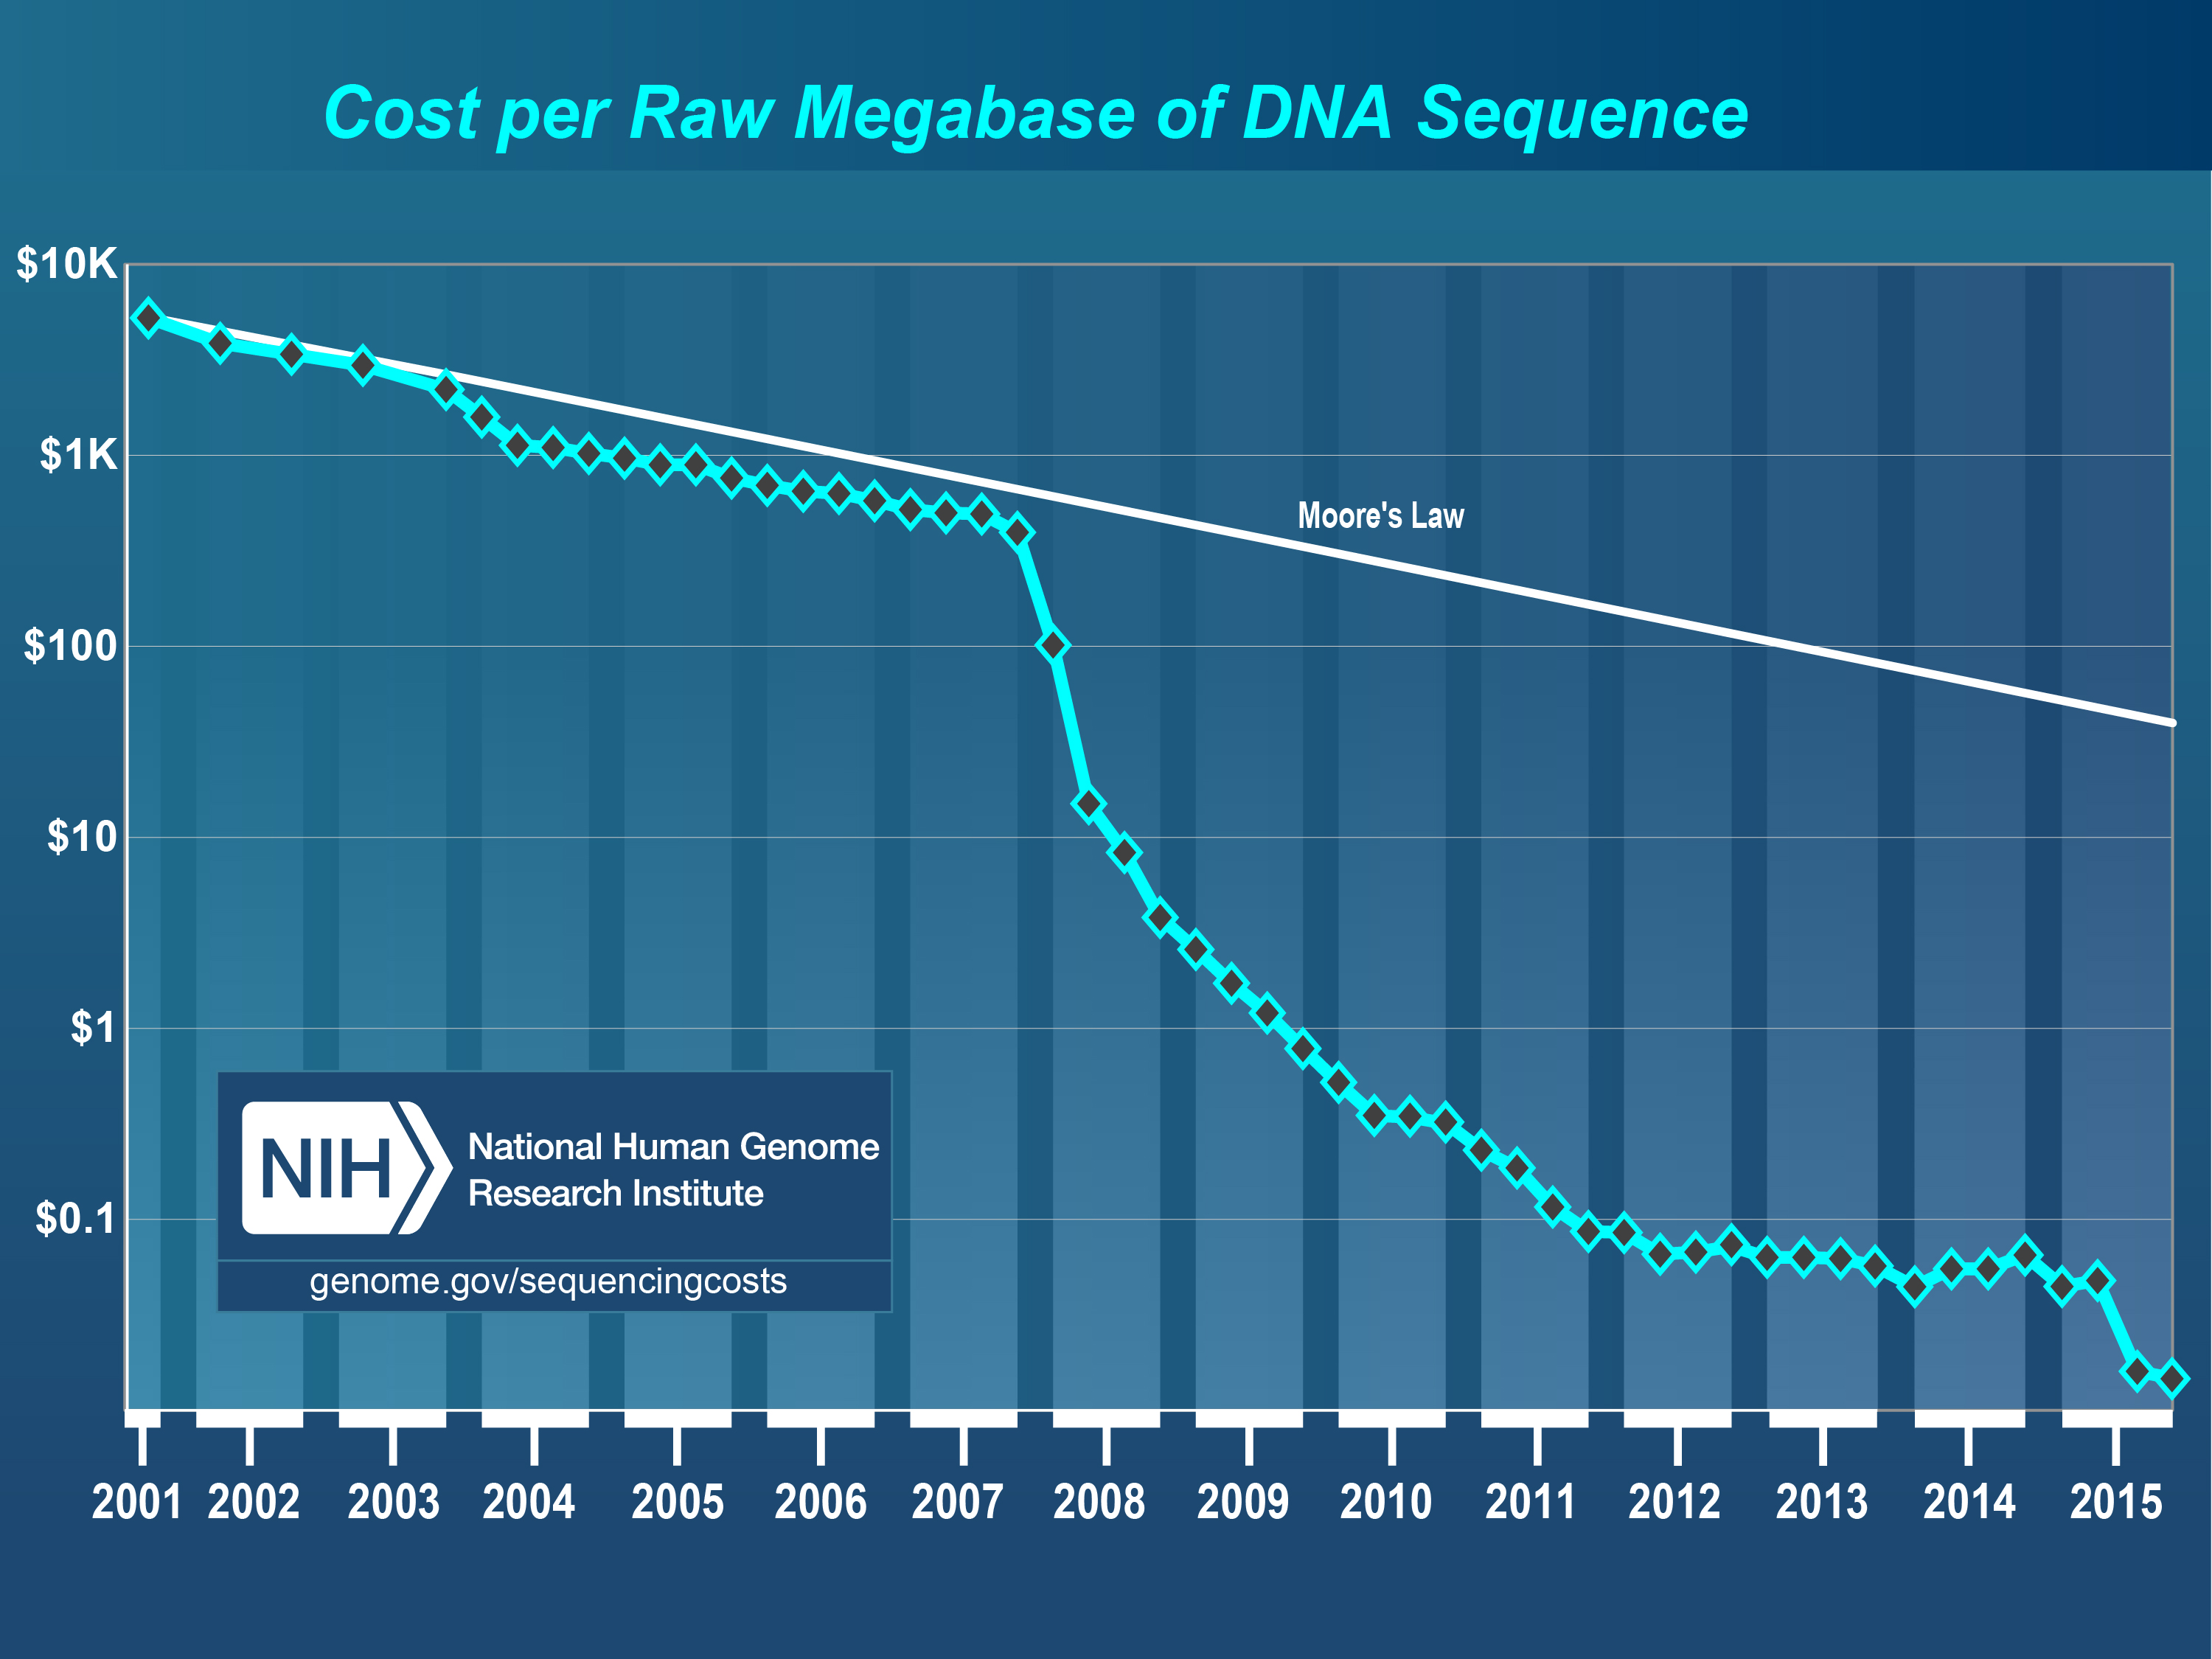
\includegraphics[width=1.0\textwidth]{costperMb2015_4.jpg}}
\end{center}
\caption[Cost per raw megabase of DNA sequence from 2001 to 2015]{Cost per raw megabase of DNA sequence from 2001 to 2015. Straight line - Moore's Law, blue curve - cost in US dollars, Y-axis scale is logarithmic. Graph reproduced from \citep{wetterstrand2016}}
\end{figure}
\begin{figure}[hb!]
\begin{center}
\makebox[\textwidth][c]{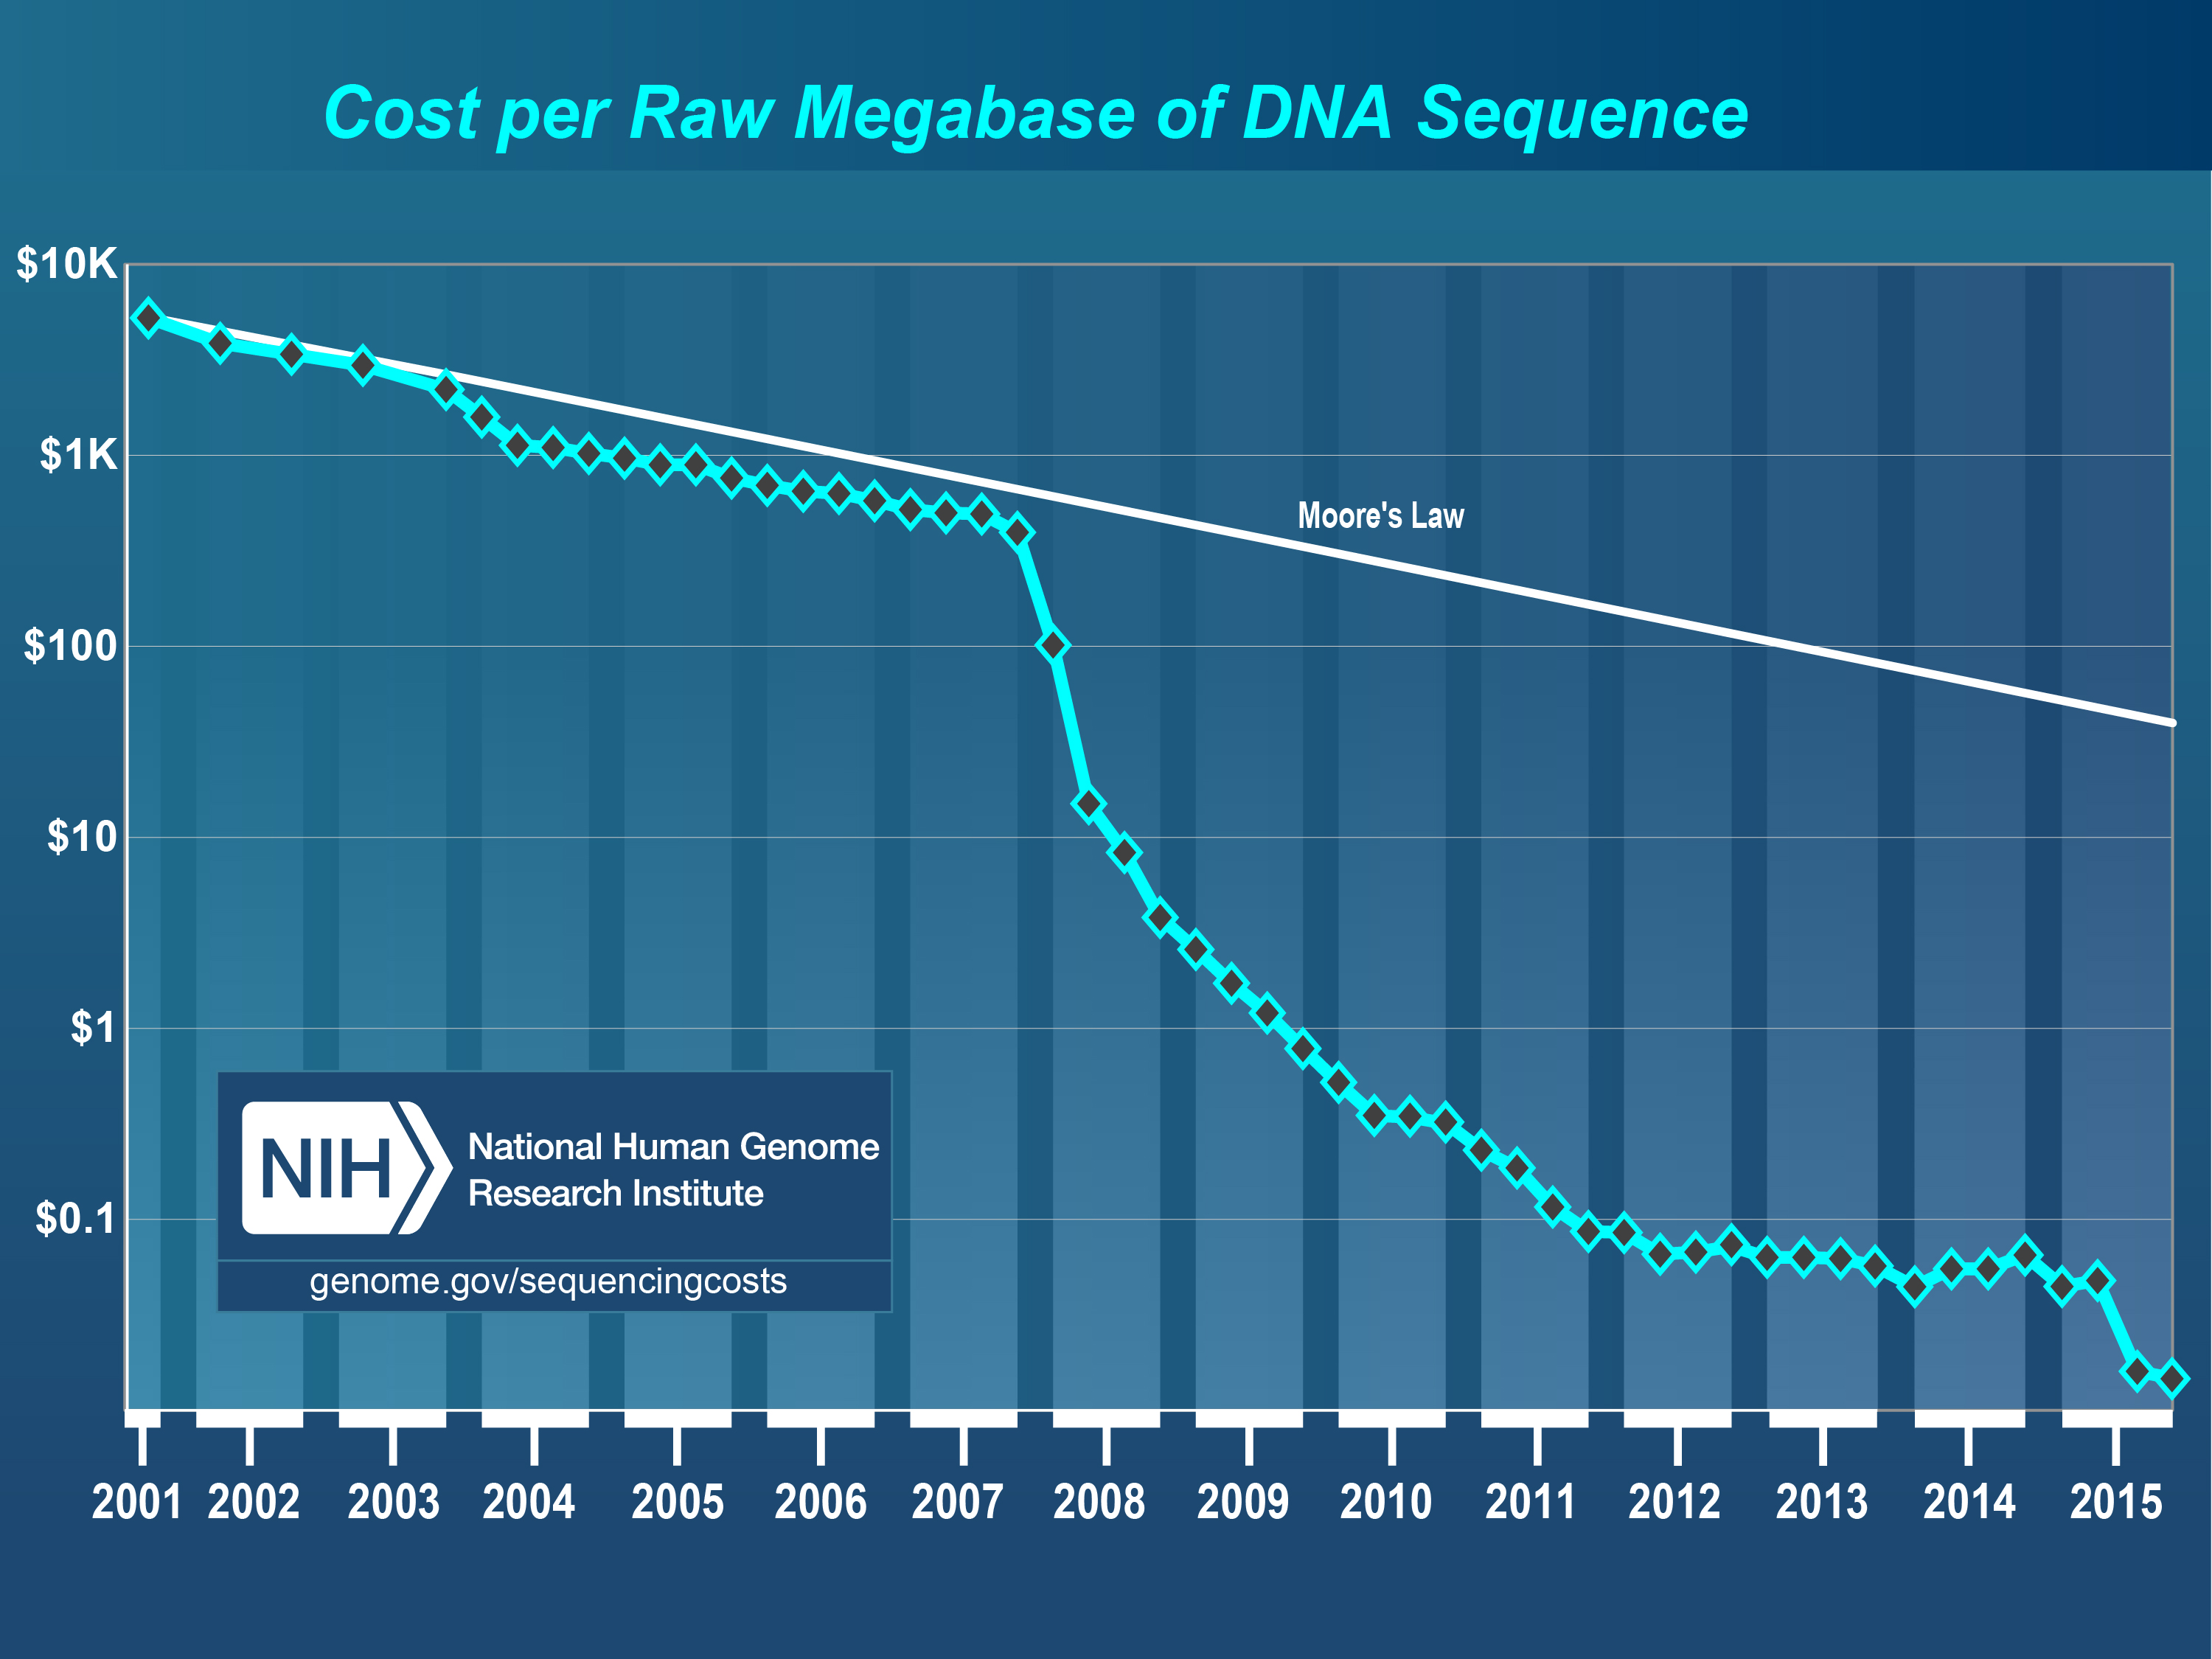
\includegraphics[width=1.0\textwidth]{costperMb2015_4.jpg}}
\end{center}
\caption[Cost per raw megabase of DNA sequence from 2001 to 2015]{Cost per raw megabase of DNA sequence from 2001 to 2015. Straight line - Moore's Law, blue curve - cost in US dollars, Y-axis scale is logarithmic. Graph reproduced from \citep{wetterstrand2016}}
\end{figure}

\chapter[Appendix]{}
\vspace*{-0.3in}
\begin{figure}[hb!]
\begin{center}
\makebox[\textwidth][c]{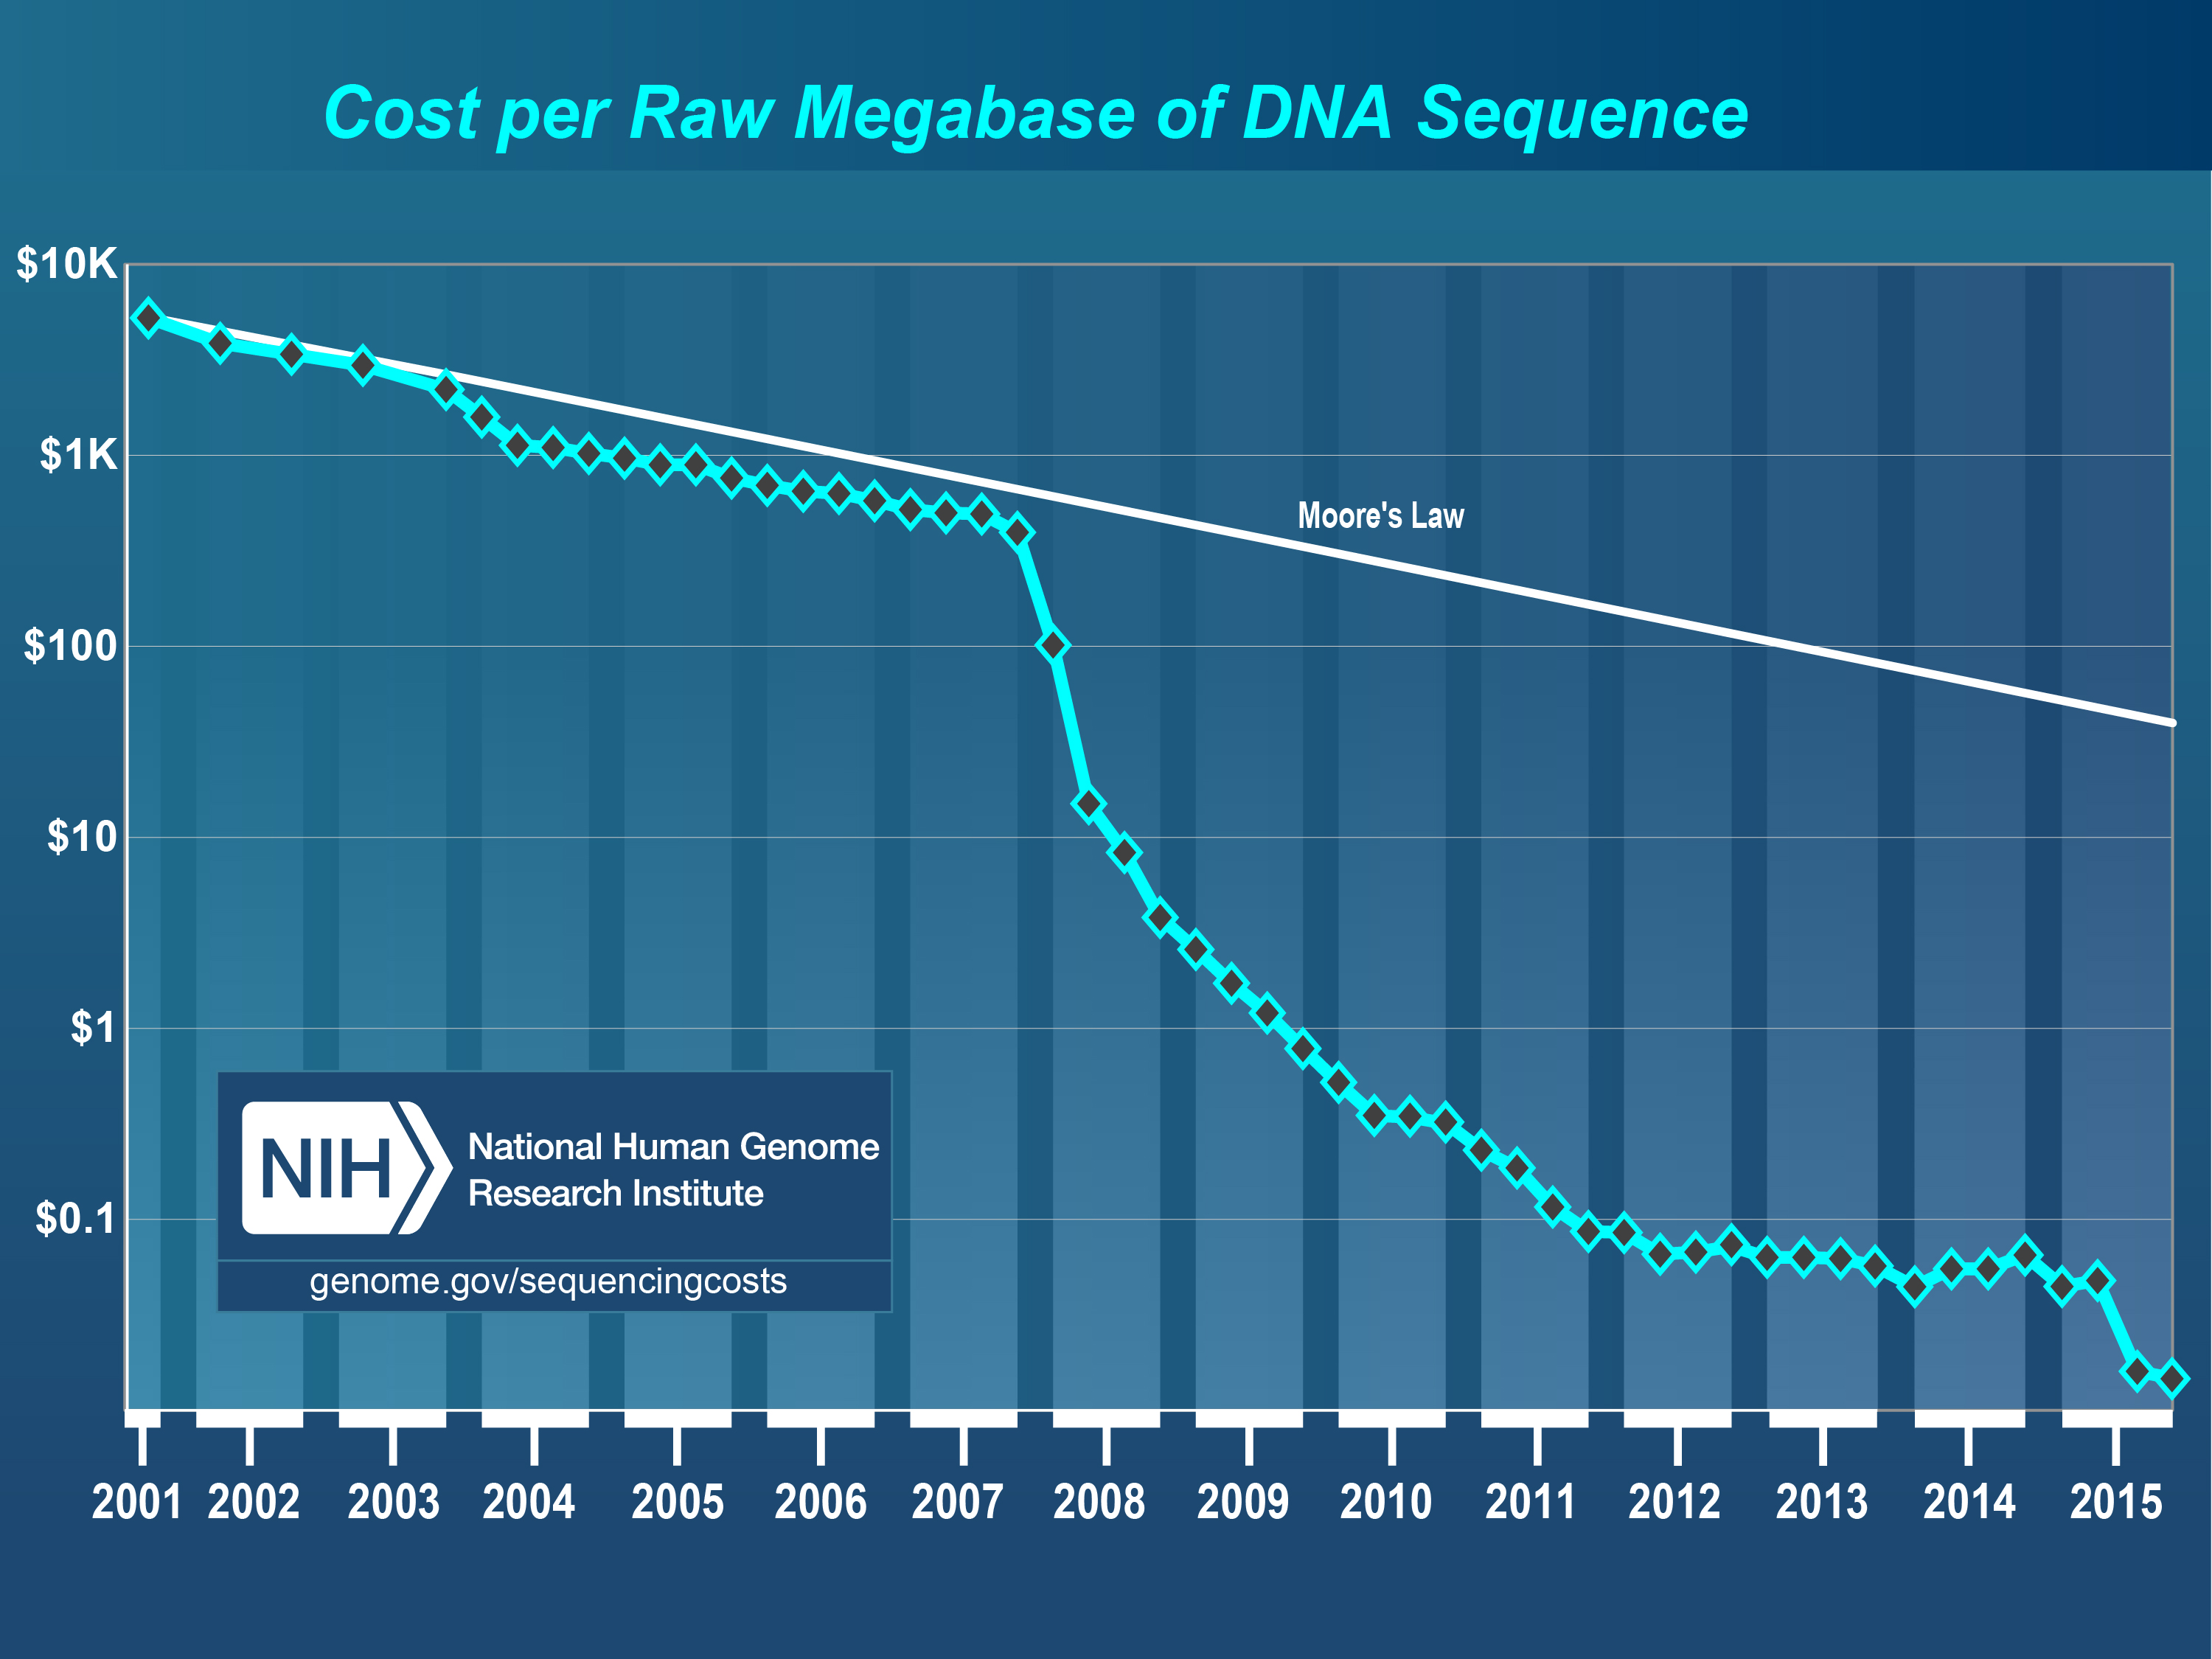
\includegraphics[width=1.0\textwidth]{costperMb2015_4.jpg}}
\end{center}
\caption[Cost per raw megabase of DNA sequence from 2001 to 2015]{Cost per raw megabase of DNA sequence from 2001 to 2015. Straight line - Moore's Law, blue curve - cost in US dollars, Y-axis scale is logarithmic. Graph reproduced from \citep{wetterstrand2016}}
\end{figure}

\chapter[Appendix]{}
\begin{figure}[hb!]
\begin{center}
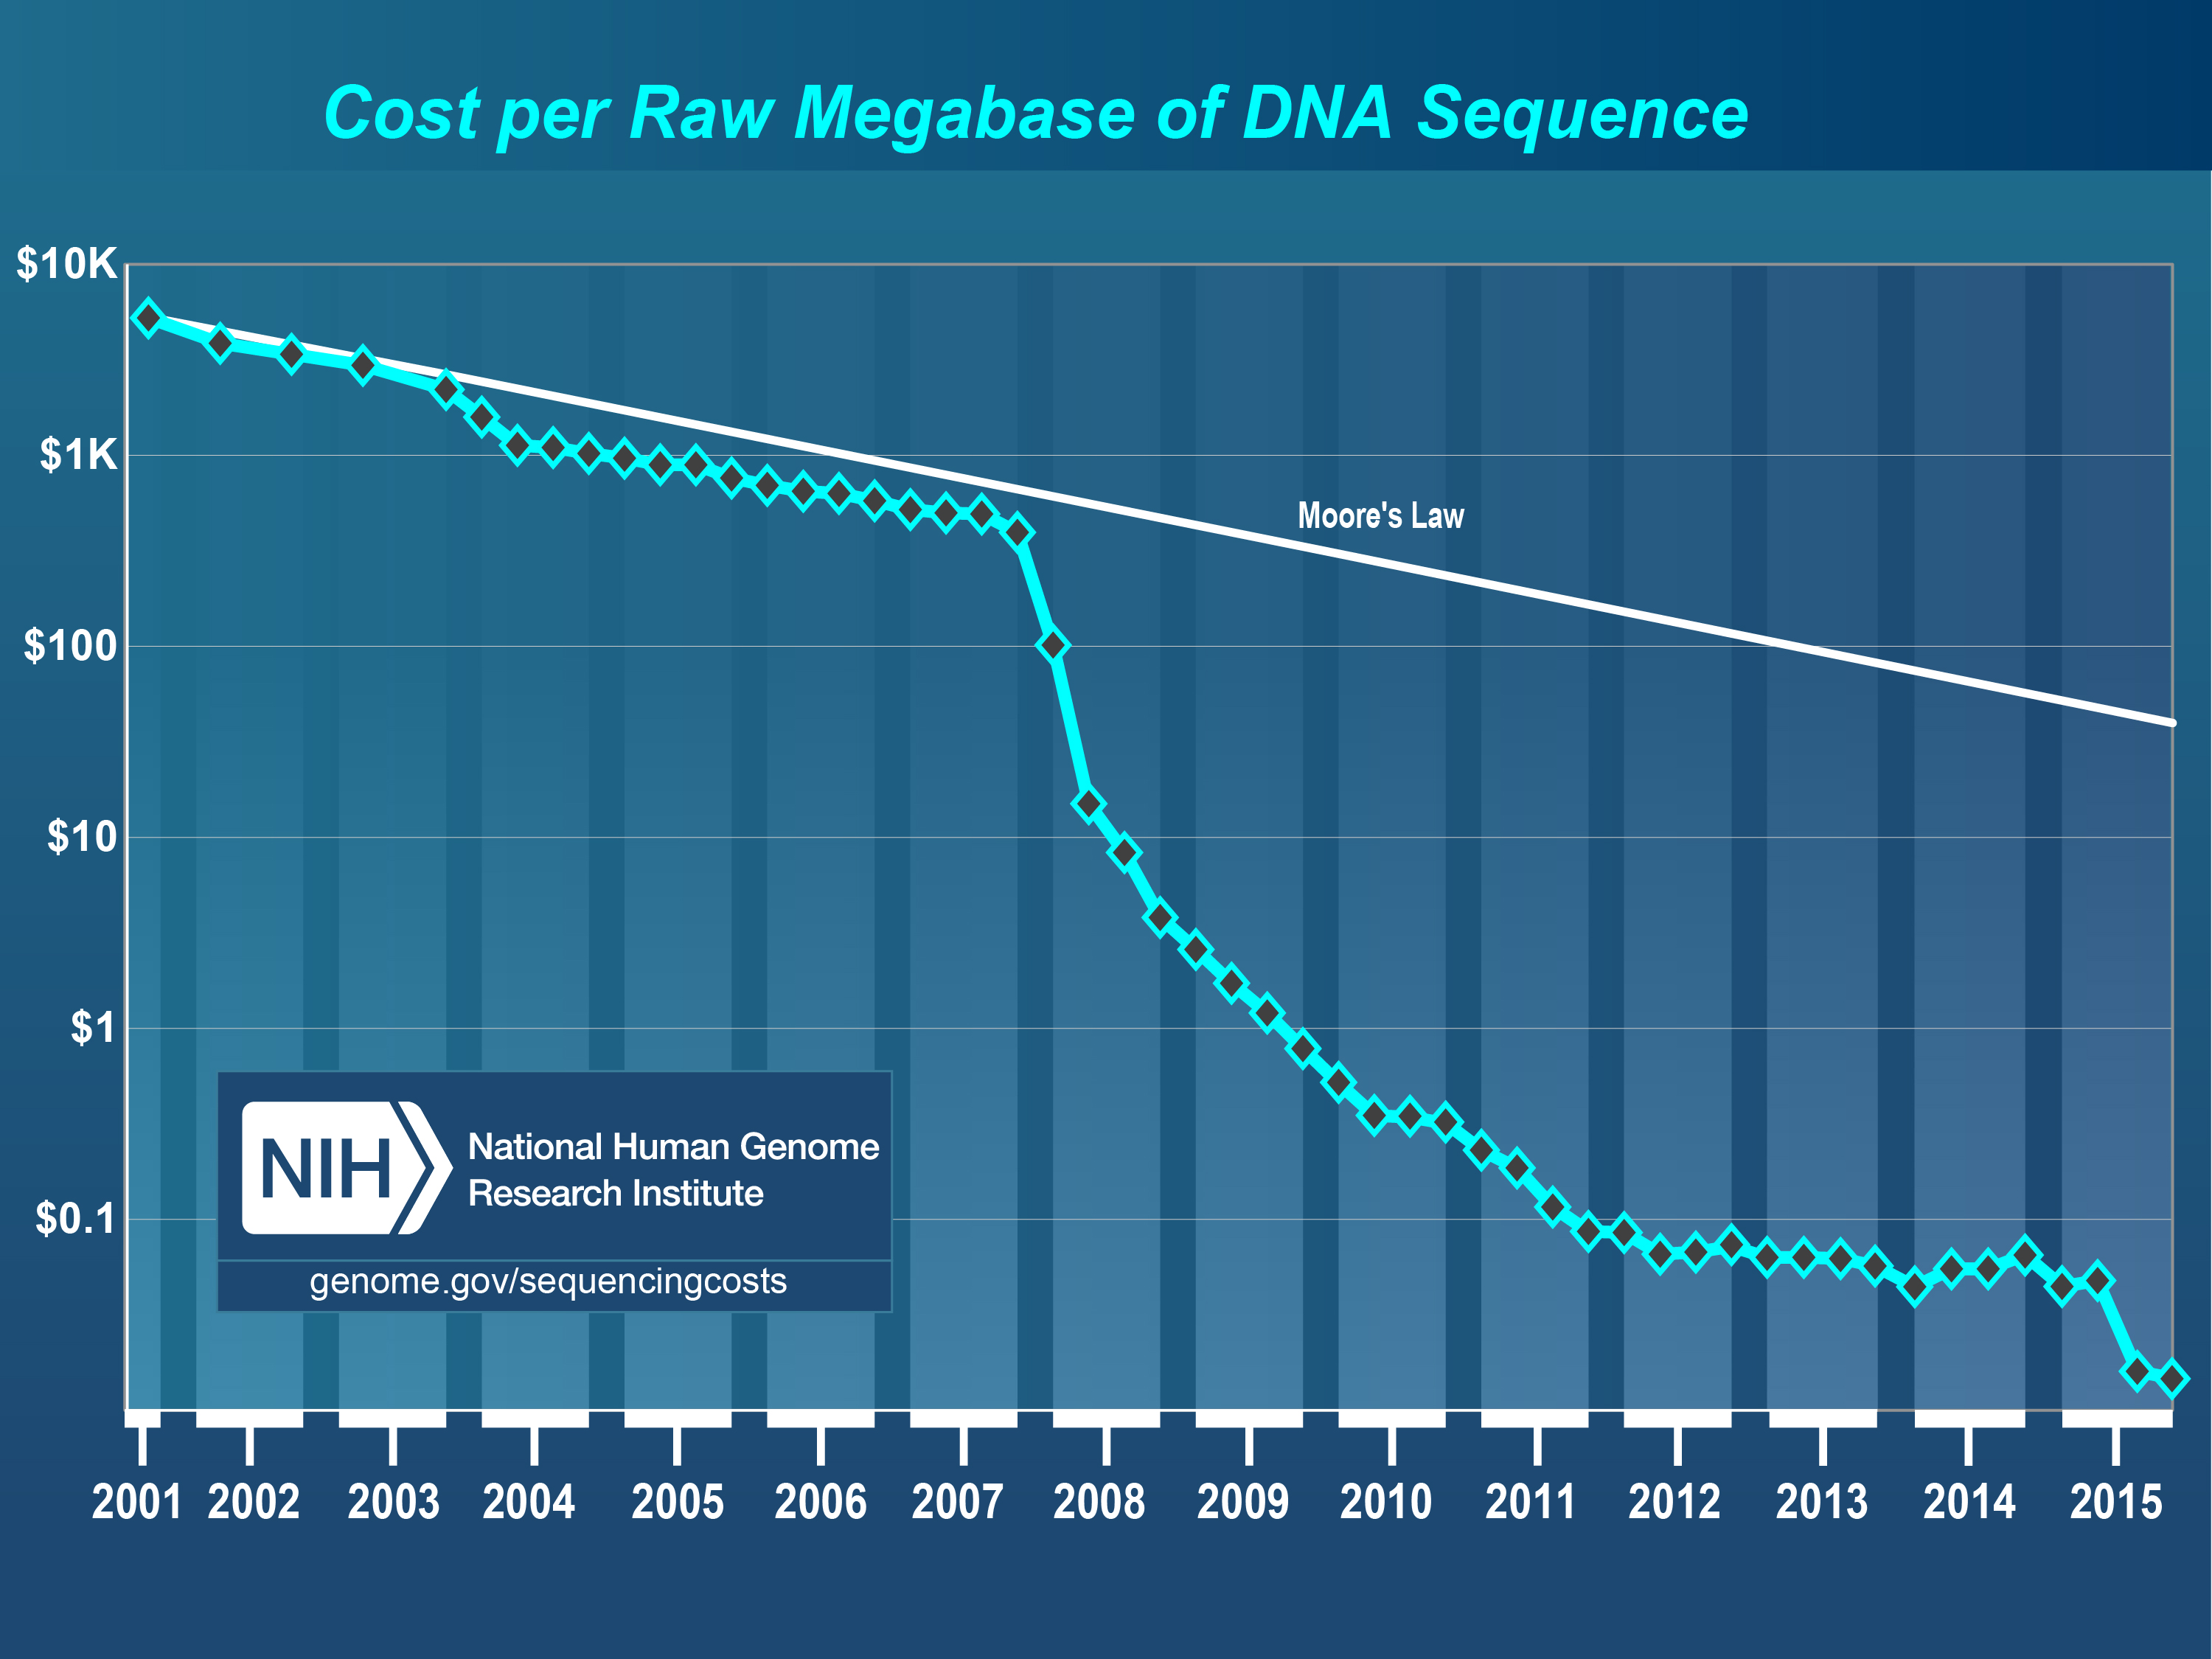
\includegraphics[scale=0.5]{costperMb2015_4.jpg}
\end{center}
\caption[Cost per raw megabase of DNA sequence from 2001 to 2015]{Cost per raw megabase of DNA sequence from 2001 to 2015. Straight line - Moore's Law, blue curve - cost in US dollars, Y-axis scale is logarithmic. Graph reproduced from \citep{wetterstrand2016}}
\end{figure}

\chapter[Appendix]{}
\begin{figure}[hb!]
\begin{center}
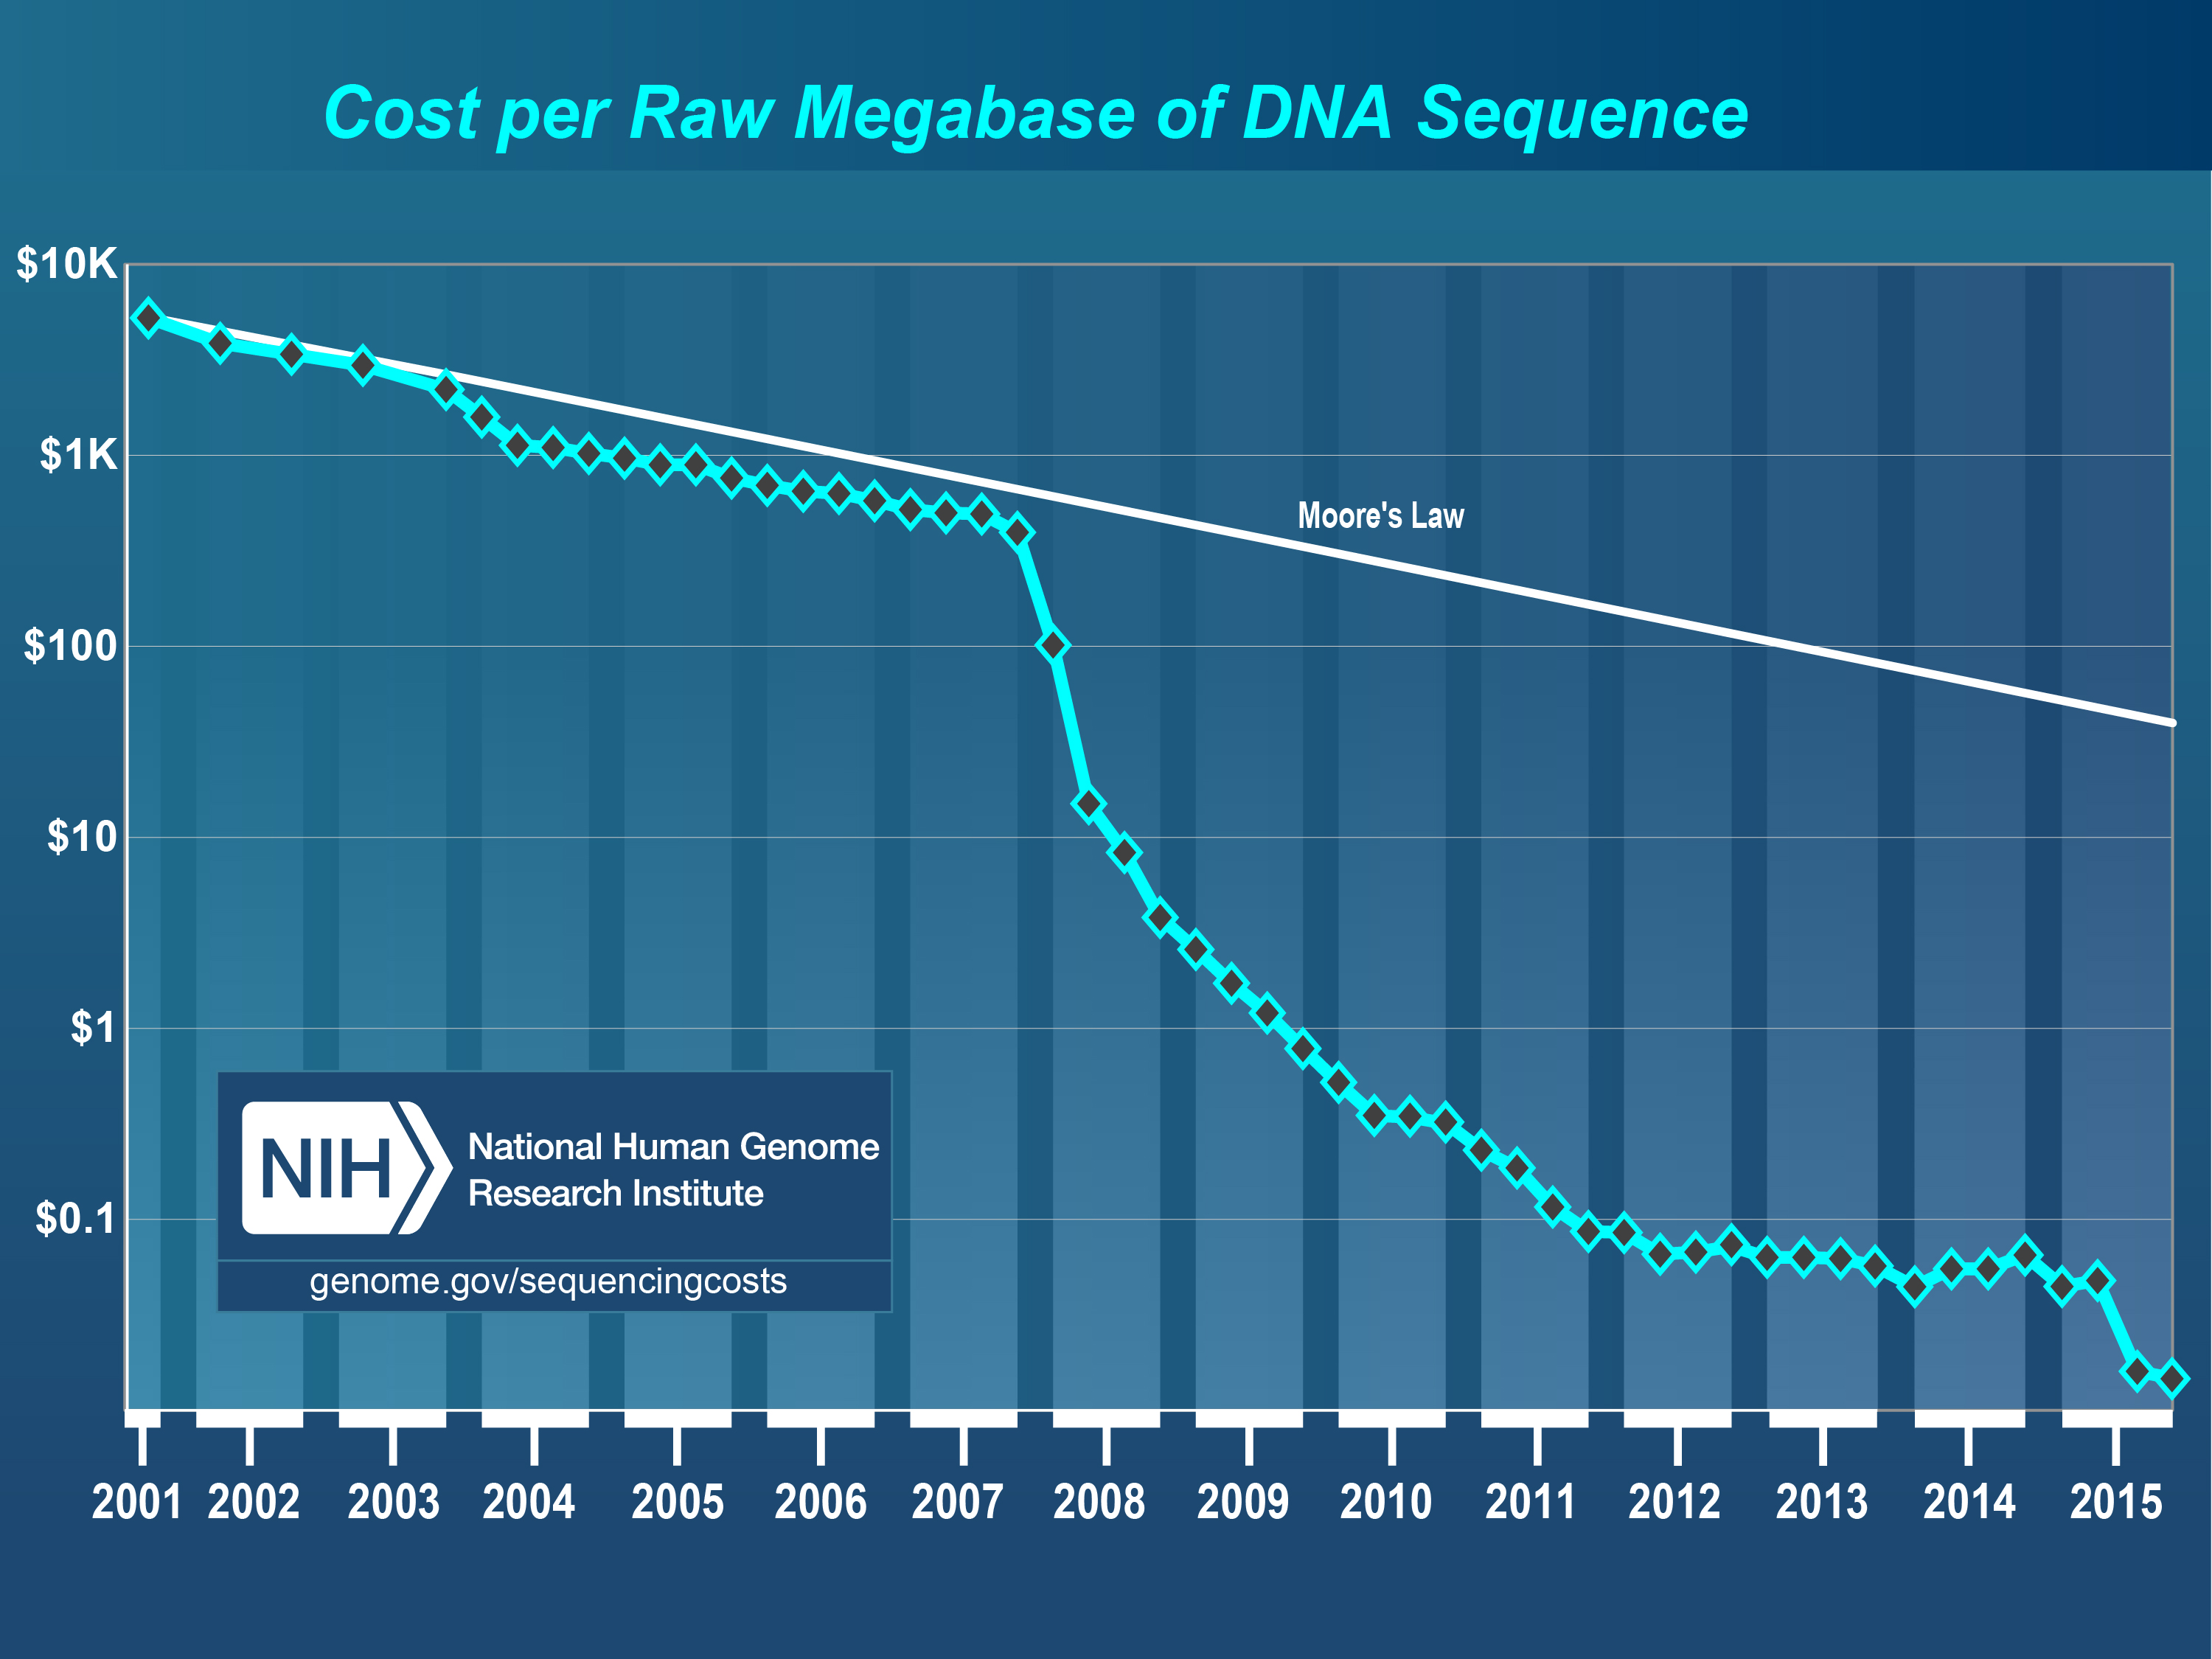
\includegraphics[scale=0.5]{costperMb2015_4.jpg}
\end{center}
\caption[Cost per raw megabase of DNA sequence from 2001 to 2015]{Cost per raw megabase of DNA sequence from 2001 to 2015. Straight line - Moore's Law, blue curve - cost in US dollars, Y-axis scale is logarithmic. Graph reproduced from \citep{wetterstrand2016}}
\end{figure}

\chapter[Appendix]{}
\begin{figure}[hb!]
\begin{center}
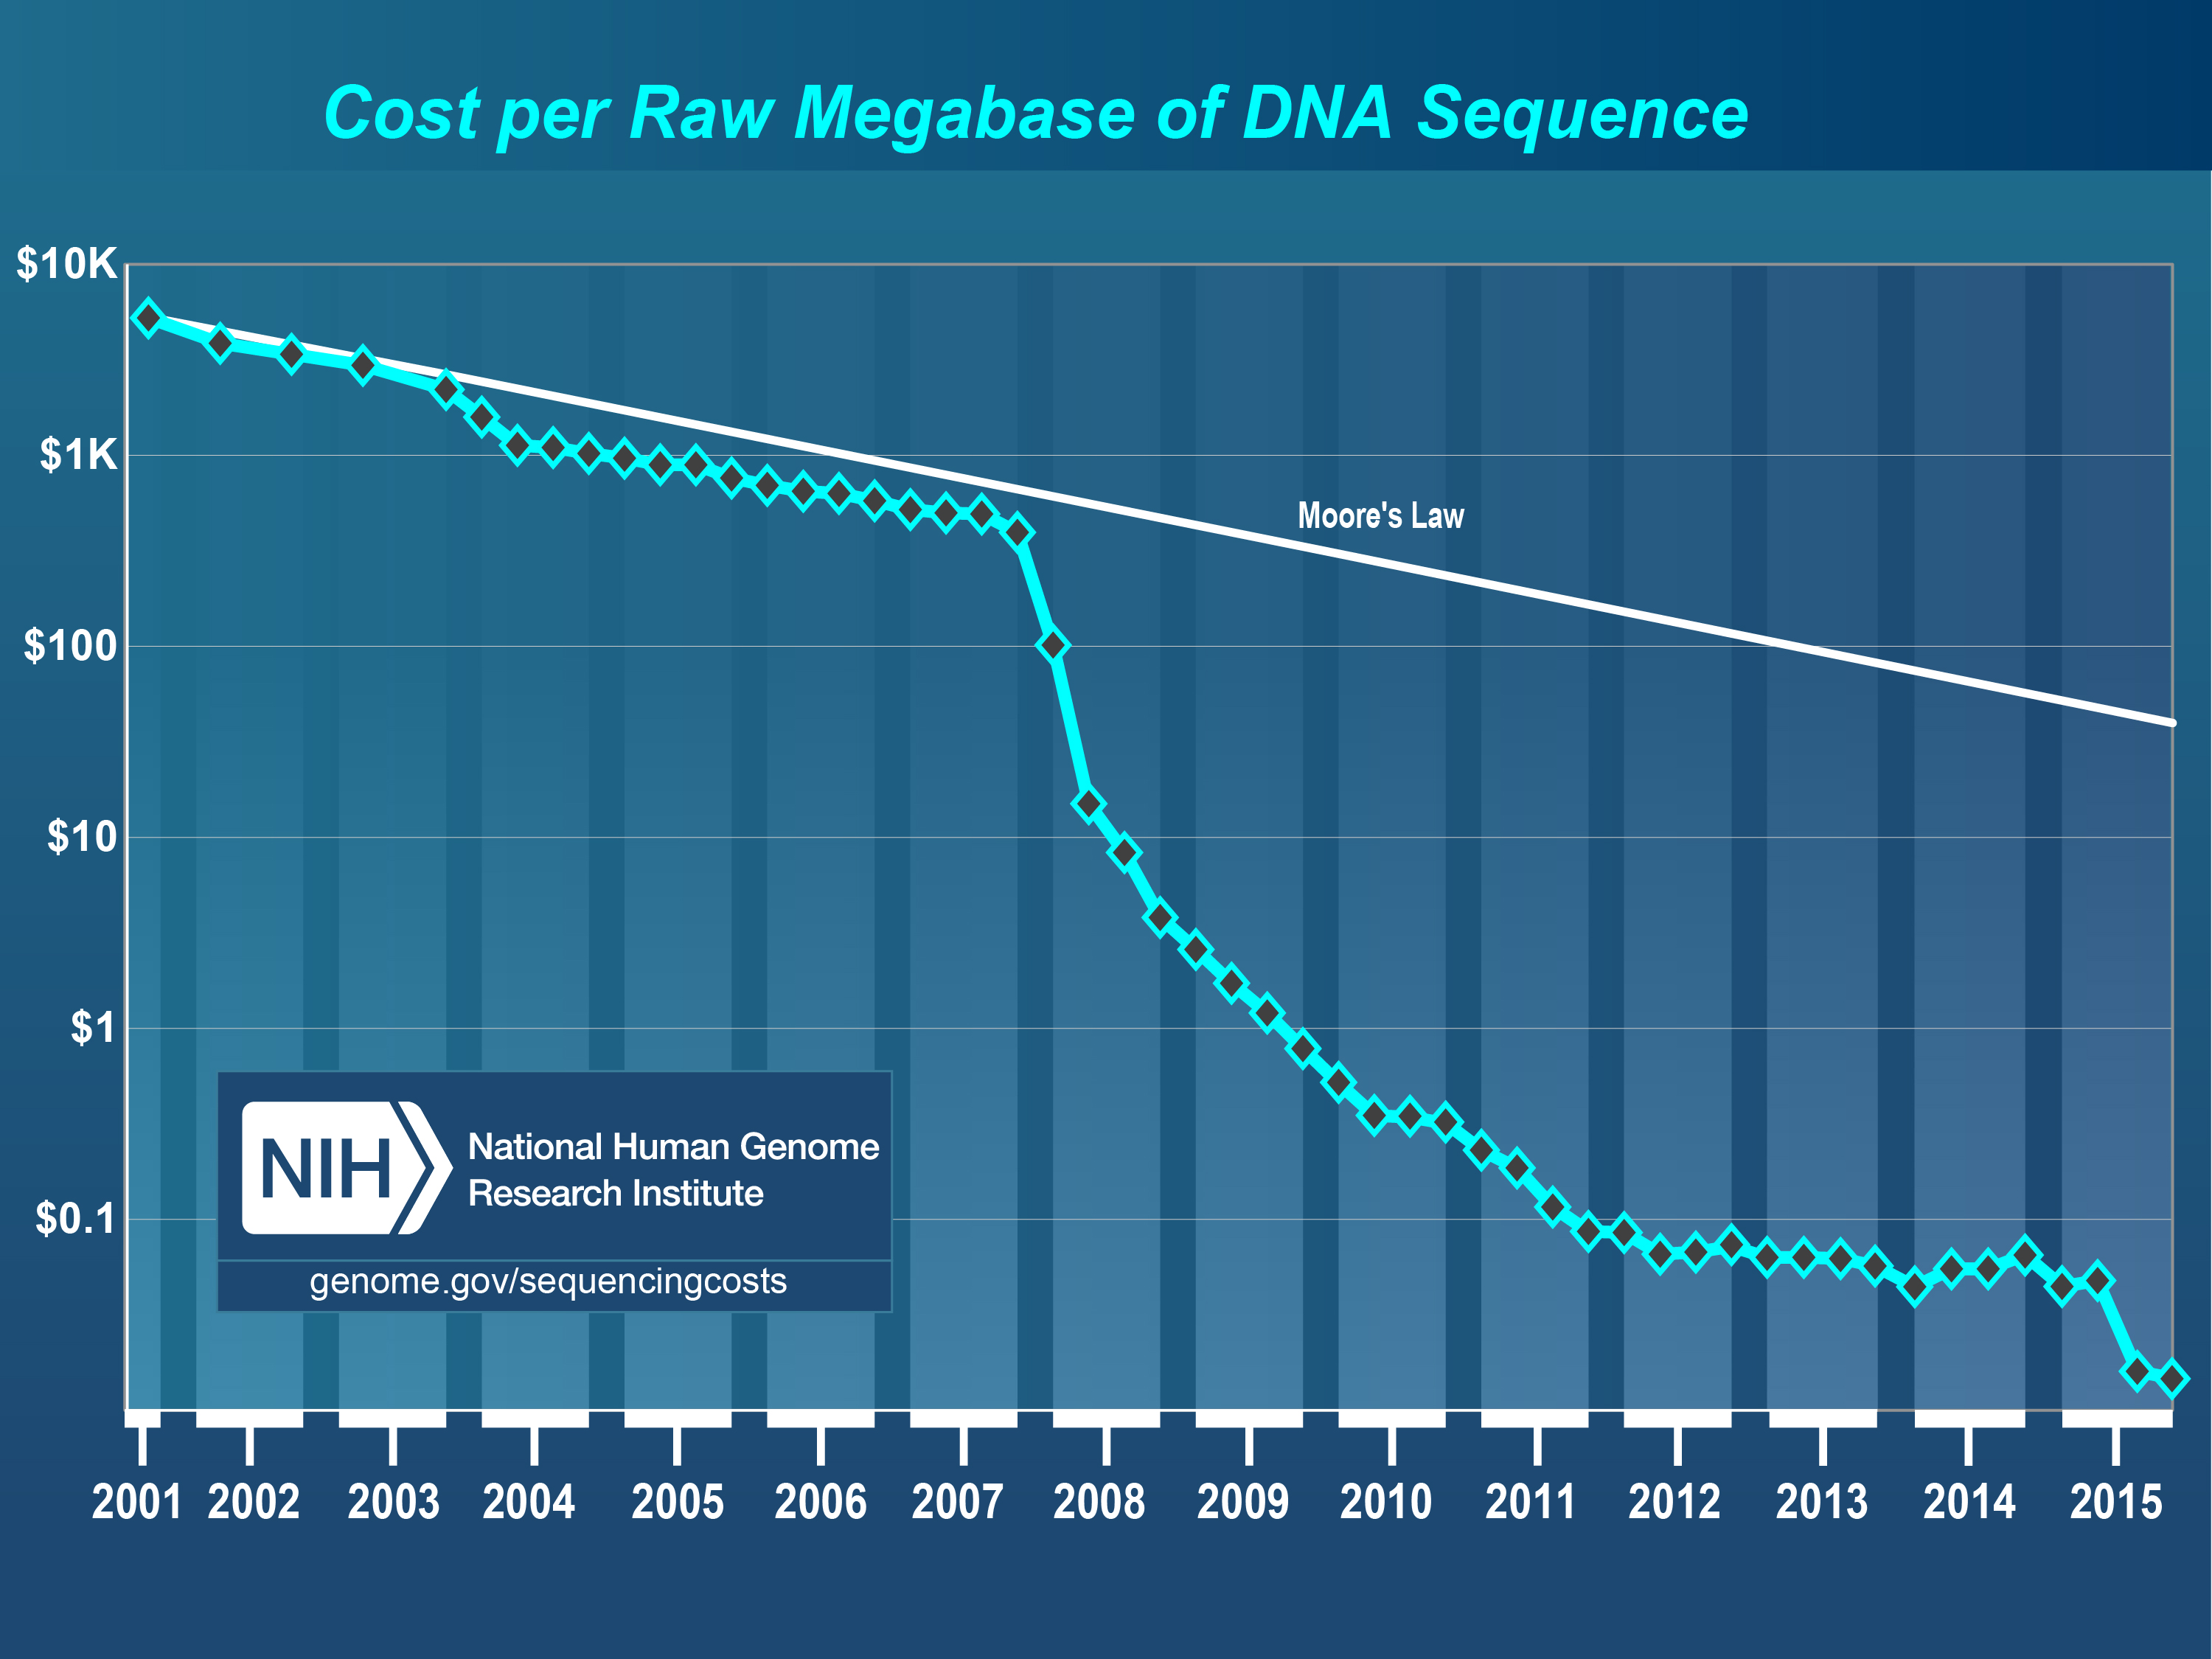
\includegraphics[scale=0.5]{costperMb2015_4.jpg}
\end{center}
\caption[Cost per raw megabase of DNA sequence from 2001 to 2015]{Cost per raw megabase of DNA sequence from 2001 to 2015. Straight line - Moore's Law, blue curve - cost in US dollars, Y-axis scale is logarithmic. Graph reproduced from \citep{wetterstrand2016}}
\end{figure}

